\documentclass[12pt]{article}
\usepackage[utf8]{inputenc}
\usepackage[pdfversion=1.7]{hyperref}
\usepackage[T1]{fontenc}
\usepackage[compress]{cite}
\bibliographystyle{naturemagnourl}
\usepackage{IEEEtrantools,stackengine}
\stackMath
\usepackage{authblk}
\usepackage{fullpage}
\usepackage[left]{lineno}
\renewcommand\linenumberfont{\normalfont\tiny}
\usepackage{amssymb,amsmath}
\usepackage{adjustbox}
\usepackage{graphicx}
% \usepackage{ltablex}
\usepackage{ragged2e}
% \usepackage{hyperref}
\usepackage{pdflscape}
\usepackage{geometry}
% \keepXColumns
\usepackage{booktabs}
\usepackage{array}
\usepackage{siunitx}
\sisetup{
    group-separator = {,},
    group-minimum-digits = 4,
    detect-all,
    detect-weight=true,
    detect-family=true,
    mode=text
  }
\usepackage{xspace}
\newcommand\ie{i.e.,\xspace}
\newcommand\eg{e.\,g.\xspace}
\newcommand\Eg{E.\,g.\xspace}
\newcommand\NB{N.\,B.\xspace}
\newcommand\BSc{B.\,Sc.\xspace}
\newcommand\MSc{M.\,Sc.\xspace}
\newcommand\PhD{Ph.\,D.\xspace}
\newcommand\etc{etc.\xspace}
\newcommand\resp{resp.\xspace}
\newcommand\cf{cf.\xspace}
\newcommand\Cf{Cf.\xspace}
\newcommand\cp{cp.\xspace}
\newcommand\etal{et\,al.\xspace}
\newcommand\page[1]{p.\,#1}
\newcommand\pages[1]{pp.\,#1}
\newcommand\pa{p.\,a.\xspace}
\newcommand\ham{a.\,m.\xspace}
\newcommand\hpm{p.\,m.\xspace}
\newcommand\UK{U.\,K.\xspace}
\newcommand\US{U.\,S.\xspace}
\newcommand\wlogenerality{w.\,l.\,o.\,g.\xspace}
\DeclareMathOperator{\logit}{logit}
\newcommand\abs[1]{\left| #1 \right|}
\newcommand{\norm}[1]{\left\lVert#1\right\rVert}
\usepackage{longtable}
\usepackage{multirow}
\usepackage[dvipsnames, table]{xcolor}
\usepackage{tikz}
\usetikzlibrary{arrows.meta, positioning}
\usepackage{minted}
% csquotes after minted (which loads fvextra) to avoid fvextra warning
\usepackage{csquotes}
\newcommand{\TODO}[1]{{\color{red}#1}}
\newcommand{\MOVE}[1]{{\color{orange}#1}}
\newcommand{\INSERT}[1]{{\color{blue}#1}}
\definecolor{darkgreen}{rgb}{0.0, 0.5, 0.0}
\newcommand{\FIX}[1]{{\color{darkgreen}#1}}
\definecolor{lightyellow}{HTML}{FFE699}
\definecolor{red_revision}{HTML}{FF0000}
\usepackage{setspace}
\doublespacing
\urlstyle{same}
\usepackage[%
  sort&compress
]{cleveref}
\Crefname{appendix}{Supplement}{Supplements}
\Crefname{figure}{Fig.}{Fig.}
\crefname{table}{Table}{Tables}
\Crefname{table}{Table}{Tables}
\usepackage{times}
\usepackage{enumerate}
\usepackage{enumitem}
\usepackage{tabularx}
\usepackage{float}
\setcounter{secnumdepth}{5}
\usepackage{subfig}
\newcommand{\figletter}[1]{{{\fontfamily{\sfdefault}\selectfont \textbf{#1}}}}
\usepackage{dcolumn}
\usepackage{rotating}
\newcommand{\mcell}[2][c]{%
  \begin{tabular}[c]{@{}#1@{}}#2\end{tabular}}
\newcommand{\mcellt}[2][c]{%
  \begin{tabular}[t]{@{}#1@{}}#2\end{tabular}}
\newcommand{\lcellt}[2][l]{%
  \begin{tabular}[t]{@{}#1@{}}#2\end{tabular}}
\newcommand{\stackedcell}[2][c]{%
  \begin{tabular}[#1]{@{}c@{}}#2\end{tabular}}
\usepackage{titlesec}
\titleformat{\subsubsection}
  {\normalfont\itshape}{\thesubsubsection}{1em}{}
\titleformat{\subsection}
  {\normalfont\bfseries}{\thesubsection}{1em}{}
\makeatletter
\renewcommand{\fps@figure}{H}
\renewcommand{\fps@table}{H}
\makeatother
\renewcommand{\arraystretch}{1.2}
\allowdisplaybreaks
\usepackage{eurosym}
\usepackage{comment}
\newcommand{\REV}[1]{\textcolor{blue}{#1}}
\usepackage{ntheorem}
\theoremseparator{:}
\newtheorem{hyp}{Hypothesis}
\newtheorem*{hyp_non}{Hypothesis}
\usepackage{makecell}
\hbadness=10000
\setlength{\emergencystretch}{3em}  
\hyphenation{                      
  an-thro-po-gen-ic
  bio-di-ver-si-ty
  e-co-sys-tem
  tax-on-o-my
  tax-o-nom-ic
  clas-si-fi-ca-tion
}

\begin{document}

%% Title page
\title{\centering\LARGE\singlespacing
Mapping direct anthropogenic drivers of biodiversity change using large language models: a systematic map protocol}

\renewcommand\Affilfont{\fontsize{9}{10.8}\selectfont}

\author[1]{Hunain Mohuiddin}
\author[1,2]{Kerstin Forster}
\author[1,2]{Stefan Feuerriegel\thanks{Corresponding author:
feuerriegel@lmu.de}}

\affil[1]{LMU Munich, Munich, Germany}
\affil[2]{Munich Center for Machine Learning, Munich, Germany}
\date{}
\maketitle
\vspace{-1cm}
\noindent\textbf{Keywords:} Global biodiversity; LLM-based systematic mapping; Anthropogenic drivers
% Type of review: Systematic Map Protocol
\newpage
\linenumbers
 
% -----------------------------------------------------------
\section*{Background}
% Describe the rationale for the review in the context of what is already known. The protocol must indicate why this study was necessary, what it aims to contribute to the field and who are the intended users of your findings. (max. 300 words)  
% ----------------------------------------------------------
Achieving the 2050 Vision of the Kunming-Montreal Global Biodiversity Framework requires understanding what drives biodiversity loss across all drivers, ecosystems, and geographies~\cite{spm_ga_ipbes_2019}. Direct anthropogenic drivers act immediately on ecosystems, species, and populations~\cite{diaz_ipbes_2015,spm_ga_ipbes_2019}, yet the scientific evidence base on these drivers remains uneven. A small subset of taxa receives the majority of research attention~\cite{troudet2017taxonomic}, and the same imbalance holds across drivers: climate change accounts for nearly 40\% of driver-related publications, while pollution is represented in fewer than 5\%~\cite{mazor_et_all_mismatch_of_policy}. Most evidence syntheses address a single driver, taxon, or region~\cite{moullec_identifying_2021,jaureguiberry_direct_2022, beckmann_conventional_2019,benitez-lopez_impact_2017,urban_accelerating_2015}, leaving the broader evidence base across drivers largely uncharacterized.

This systematic map will apply a broad search strategy for biodiversity change and direct anthropogenic drivers to screen over 2.4 million candidate bibliographic records. Following the Intergovernmental Science-Policy Platform on Biodiversity and Ecosystem Services (IPBES) conceptual framework~\cite{diaz_ipbes_2015}, eligible records will be coded to produce a structured evidence base across drivers, threats, geography, ecosystems, study attributes, and taxa. The rapidly expanding biodiversity literature makes comprehensive manual synthesis increasingly challenging~\cite{nunez-mir_automated_2016}; therefore, this map will use Large Language Models (LLMs) to automate screening and coding within the Collaboration for Environmental Evidence (CEE) systematic mapping framework. The map will help biodiversity researchers and policymakers identify evidence gaps and research priorities across direct anthropogenic drivers.

% The rapidly expanding biodiversity literature makes comprehensive manual synthesis increasingly challenging~\cite{nunez-mir_automated_2016}; therefore, this map will use Large Language Models (LLMs) to automate screening and coding within the Collaboration for Environmental Evidence (CEE) systematic mapping framework, with deviations documented and supported by consistency checking~\cite{CEE_Guidelines_5_1_2022}.

% -----------------------------------------------------------
\subsection*{Theory of Change or Causal Model}
% Provide a theory of change and/or conceptual model that describes the hypothesised link(s) between the intervention/exposure to the outcome(s). Use either text or attach graphic as an additional file. (max. 100 words)
% -----------------------------------------------------------
This systematic map does not evaluate interventions and does not construct a causal model. Following the IPBES conceptual framework~\cite{diaz_ipbes_2015}, it characterizes the scientific evidence base on direct anthropogenic drivers of biodiversity change. The map draws on this framework to define the exposure (direct anthropogenic drivers) and outcome (biodiversity change), as illustrated in Supplementary Figure~\ref{figure:conceptual_model}.

% -----------------------------------------------------------
\section*{Stakeholder Engagement}
%% Proceed submission guidelines: Describe the role of stakeholders in the formulation of the question and this protocol and any further role throughout the review process. (Max 150 words)
% -----------------------------------------------------------
No formal external stakeholder consultation will be conducted. However, screening and coding outputs will be compared against labels from previously published sources on biodiversity change through the consistency checking procedures described in this protocol.

% -----------------------------------------------------------
\section*{Objectives and Review Question}
%% Proceed submission guidelines: State the primary review question (and secondary questions when applicable). (Max 100 words)
% -----------------------------------------------------------
The objective of this systematic map is to collect, code, and
characterize the scientific evidence on the direct anthropogenic drivers of biodiversity change, with primary analytical focus on biodiversity loss. The map is guided by two overarching questions:

\begin{enumerate}
  \sloppy 
  \item What scientific evidence is available on the direct anthropogenic drivers of biodiversity change?
  \item How is this evidence characterized across direct anthropogenic drivers, specific threats, geography, ecosystems, study attributes, and taxa?
\end{enumerate}

% -----------------------------------------------------------
\subsection*{Definitions of the Question Components}
%% Break down and summarise question key elements e.g. population, intervention(s)/exposure(s), comparator(s), and outcome(s).(Max 150 words)
% -----------------------------------------------------------
The review questions are defined using the Population, Exposure, and Outcome (PEO) framework.

\emph{Population:} This map broadly covers total biodiversity, the variability among living organisms from all sources~\cite{CBD1992}. No geographic or taxonomic restriction is applied; all taxonomic groups, ecosystems, and geographies will be coded using pre-defined classification schemes~\cite{diaz_ipbes_2015,iucn_threats_classification_2022,data_ipbes_geo,keith2022function_get,GBIFBackboneTaxonomy_general}.

\emph{Exposure:} The exposure comprises any direct anthropogenic driver acting on biodiversity, classified using the five IPBES driver categories~\cite{diaz_ipbes_2015} and further resolved using the International Union for Conservation of Nature (IUCN) Threats Classification~\cite{iucn_threats_classification_2022}.

\emph{Outcome:} The outcome is reported biodiversity change at genetic, species, community, or ecosystem level. The primary focus is negative change.
% -----------------------------------------------------------
\section*{Search Strategy}
%% Proceed submission guidelines: Detail the planned search strategy to be used. Sources of articles searched should capture both conventionally published scientific literature and gray literature using a combination of databases, search engines and specialist websites (may also be informed by stakeholders) or limitations should be fully justified. Provide information about the sources to be searched and search options selected, together with dates of search and any language limitations. All search terms and search strings, with Boolean operators (‘AND’, ‘OR’ etc.) and wildcards, should be clearly stated for each major source (e.g. databases, search engines) so that the exact search is replicable by a third party but search terms for minor sources (e.g. specialist websites), can be left flexible. Some of these elements may be detailed in 8.1-8.3 below.
%% (Max 250 words)
% -----------------------------------------------------------
The literature search will be conducted on Web of Science Core Collection (WoS), with publication years 2000--2026; records with publication-date metadata after 30~April~2026 will be excluded at the point of export. The search string is designed to prioritize recall over precision, capturing a broad corpus (see Table~\ref{table:wos_search_components}). It comprises five components combined using \texttt{AND}: a publication-type filter (A); a scientific disciplines filter via WoS subject categories (B); a change/assessment terms block (C); five driver-specific sub-strings, one per IPBES direct driver category, combined using \texttt{OR} and adopted from a prior rapid evidence assessment~\cite{jaureguiberry_direct_2022} (D); and a publication-year filter (E).

% table:wos_search_components
\newgeometry{top=0.8cm, bottom=1.5cm, left=1cm, right=1cm}
\thispagestyle{plain}
\begin{landscape}

\begin{table}[p]
\renewcommand{\arraystretch}{1.15}
\setlength{\tabcolsep}{3pt}
\centering
\tiny
\begin{tabularx}{\linewidth}{|>{\raggedright\arraybackslash}p{0.13\linewidth}
                             |>{\raggedright\arraybackslash}p{0.06\linewidth}
                             |>{\raggedright\arraybackslash}p{0.22\linewidth}
                             |>{\raggedright\arraybackslash}p{0.06\linewidth}
                             |>{\raggedright\arraybackslash}X|}
\hline
\textbf{Component} &
\textbf{Operator} &
\textbf{What this block does} &
\textbf{WoS field} &
\textbf{Search string} \\
\hline

(A) Publications &
AND &
Limit results to articles only.  &
DT &
\texttt{DT=(Article)} \\
\hline

(B) Scientific disciplines &
AND &
Limits results to relevant Web of Science Categories to keep retrieval manageable. &
WC &
\texttt{WC=("Biodiversity Conservation" OR "Ecology" OR "Environmental Sciences" OR "Environmental Studies" OR "Marine \& Freshwater Biology" OR "Fisheries" OR "Oceanography" OR "Forestry" OR "Water Resources" OR "Agronomy" OR "Geosciences, Multidisciplinary" OR "Meteorology \& Atmospheric Sciences" OR "Plant Sciences" OR "Zoology" OR "Remote Sensing" OR "Multidisciplinary Sciences")} \\
\hline

(C) Change / assessment / monitoring terms &
AND &
Ensures retrieved records include language indicating measured change or assessment/monitoring (e.g., loss/change, impacts/pressures, trends/responses, risk, monitoring). &
TS &
\texttt{TS=((loss* NEAR/3 (habitat* OR biodiversit* OR species OR population* OR "ecosystem service*" OR ecosystem* OR forest* OR coral* OR mangrove* OR reef* OR wetland* OR bird* OR mammal* OR plant*)) OR change* OR reference* OR indicator* OR impact* OR effect* OR pressure* OR trend* OR response* OR status OR pattern* OR assessment* OR monitor* OR risk* OR driver*)} \\
\hline

\multicolumn{5}{|l|}{\textbf{(D) Direct drivers of anthropogenic biodiversity change (driver sub-strings combined with OR within TS)}} \\
\hline

(D1) Land/sea use change &
OR &
Terms capturing land/sea use change and habitat modification. &
TS &
\texttt{(("land use chang*" OR "land cover chang*" OR "land* system* chang*" OR "land* chang*" OR "land* degradation" OR "land* conversion" OR "land management") OR ((marine OR ocean OR sea*) AND use AND change*) OR ("habitat loss*" OR "habitat degradation*" OR "habitat chang*" OR "habitat conversion" OR "habitat modification*" OR "habitat fragmentation" OR "habitat management") OR (biofuel* OR biogas*) OR ((residential OR urban* OR cities OR housing OR commercial OR industrial OR touris* OR recreation*) AND (extent OR area OR cover* OR proportion* OR percentage*) AND (develop* OR expan* OR increas*)) OR (deforestation OR afforestation OR "wood plantation*" OR "forest* plantation*" OR "pulp* plantation*") OR ((aquaculture* OR agricultur* OR crop* OR "cultivated area*" OR farmland OR pasture) AND (develop* OR expan* OR increas* OR intensification OR extensification OR abandon* OR chang*)) OR (livestock AND (farm* OR ranch* OR graz* OR densit*)) OR (energy AND (drill* OR min* OR quarry*)) OR (((transport* OR service) AND (network* OR corridor* OR infrastructure*)) OR road* OR rail* OR "ship* lane*" OR "flight path*") OR ("system* modification*" OR (dams OR (water AND (management OR use))))) } \\
\hline

(D2) Direct Exploitation and Resource Extraction &
OR &
Terms capturing extraction/harvest/withdrawal of biological and abiotic resources, including fishing and logging. &
TS &
\texttt{(((((natur* AND resource*) OR material* OR (biomass OR "fossil fuel*" OR ore* OR mineral*)) OR ((biological AND resource*) OR wildlife OR animal* OR plant* OR population*) OR water) AND ((overextraction OR overexploitation) OR (extraction OR exploitation OR withdraw*) OR depletion OR (hunting OR collect* OR gather* OR poaching OR "bush meat*"))) OR ((forest* OR wood OR timber*) AND (harvest* OR logging*)) OR (soil* AND (erosion OR acidification OR degradation)) OR (fisher* OR fishing OR (bycatch OR by-catch))} \\
\hline

(D3) Climate change &
OR &
Terms capturing climate change and associated climatic stressors and impacts. &
TS &
\texttt{("climat* change" OR "chang* climat*" OR ("increase* temperature*" OR "thermal alteration" OR "global warming") OR (chang* AND precipitation*) OR ((extreme OR severe) AND (weather OR temperature OR precipitation OR climat*)) OR heatwave* OR drought* OR storm* OR flood* OR (UV OR ultraviolet) OR "sea level rise" OR "soil salinization" OR ("habitat shift*" AND climate) OR ("habitat alteration" AND climate) OR ((consumptive OR human OR agricultural) AND "water stress"))} \\
\hline

(D4) Pollution &
OR &
Terms capturing pollution and contaminants across environmental media (soil/water/air). &
TS &
\texttt{((pollut* OR contamin* OR emission* OR spill-over* OR disposal* OR deposition* OR load* OR dump* OR discharge*) OR ((noise OR light OR gas* OR particle* OR particulate* OR nitrogen OR sulphur* OR phosphor* OR waste* OR garbage OR sewage OR pesticide* OR fertilizer* OR nutrient* OR "oil spill*" OR metal OR salinization OR salinisation OR acidification OR solid OR plastic OR mercury OR nutrient* OR pollutant*) AND (soil OR water OR ocean OR marine OR atmosphere OR air)) OR ((industrial OR military OR agricultur* OR forest*) AND effluent*))} \\
\hline

(D5) Invasive alien species &
OR &
Terms capturing invasive alien species introductions and biological invasions. &
TS &
\texttt{(((invasive OR invasion) AND (alien OR exotic OR non-native OR pest* OR disease) AND species) OR "biological invasion*" OR (introduc* AND (species OR material)))} \\
\hline

(E) Publication year &
AND &
Restricts results to the selected publication year range. &
PY &
\texttt{PY=2000--2026} \\

\hline

\end{tabularx}
\caption{Search string components used in Web of Science: Components (A)--(E) are combined using \texttt{AND}. Within \texttt{TS}, the five direct driver sub-strings (D1--D5) from \cite{jaureguiberry_direct_2022} are combined using \texttt{OR}. Component~(E) applies the WoS publication-year filter \texttt{PY=2000--2026}; because WoS publication-year filtering does not express a day/month cutoff, records with publication-date metadata after 30~April~2026 will be excluded at the point of export. A preliminary feasibility check conducted on 02~May~2026 yielded over 2.4~million unique records after deduplication, confirming the scale of the corpus to be screened and coded.}


\label{table:wos_search_components}
\end{table}
\end{landscape}
\restoregeometry


% -----------------------------------------------------------
\subsection*{Bibliographic Databases}
% Provide details of all bibliographic databases to be searched, including database names accessed, institutional subscriptions (or date ranges subscribed for each database), search options (e.g. ‘topic words’ or ‘full text’ search facility), languages and search strings (Max 250 words)
% -----------------------------------------------------------
The search will be executed on the WoS Core Collection. Throughout the search, no language restrictions will be applied. Gray literature is excluded in this systematic map; processing of gray literature at this corpus scale falls outside the scope of the LLM pipeline. This is acknowledged as a limitation of the search coverage.

% -----------------------------------------------------------
\subsection*{Web-Based Search Engines}
% Provide details of all web-based search engines to be searched, including names, languages and search strings. (Max 250 words)
% -----------------------------------------------------------
No web-based search engines will be searched.

% -----------------------------------------------------------
\subsection*{Organizational Websites}
% Provide details of all organizational websites to be searched, including names, languages and search strings. (Max 250 words)
% -----------------------------------------------------------
No organizational websites will be searched.
% -----------------------------------------------------------
\subsection*{Comprehensiveness of the Search}
% Describe the process by which the comprehensiveness of the search strategy was assessed (i.e. by percentage retrieval of an independently assembled list of benchmark articles known to be eligible). Describe the outcome of the assessment and your subsequent action if necessary. (Max 250 words)
% -----------------------------------------------------------
Comprehensiveness was assessed against an \emph{a priori} test list of 581 publications compiled from five published sources (three meta-analyses, a rapid evidence assessment, and a systematic map protocol) on direct drivers of biodiversity loss~\cite{moullec_identifying_2021, jaureguiberry_direct_2022, beckmann_conventional_2019, benitez-lopez_impact_2017, urban_accelerating_2015} and the IPBES Global Assessment chapters on direct drivers (sections 2.1.12--2.1.17)~\cite{balvanera_chapter_2019}. Together, these sources span all five IPBES direct driver categories.

The test list was assembled by extracting reference lists from each source and excluding gray literature and records not indexed in WoS, yielding 581 records from an initial 791 candidates. The final search string retrieved 497 of these records, yielding source-specific recall ranging from 71.43\% to 97.32\% and an overall recall of 85.54\%. 

% -----------------------------------------------------------
\subsection*{Search Update}
% Describe any plans to update the searches during the conduct of the review (Max 250 words)
% -----------------------------------------------------------
No search updates are planned. 
% -----------------------------------------------------------
\section*{Screening Strategy}
% Describe the methodology for screening articles/studies for eligibility (Max 250 words)
% -----------------------------------------------------------
The literature search will retrieve over 2.4 million bibliographic records spanning all five direct anthropogenic drivers of biodiversity change. All eligibility screening decisions will be made by GPT-5-nano (version \texttt{2025-08-07}). Prompts and the reasoning effort parameter will be finalized on the training and development splits of the validation datasets and frozen prior to full-corpus application; prompts tuning and freezing procedure is described in \hyperref[sec:prompts_configs] {Supplementary Text S2}.

The model will apply a four-question procedure (\texttt{Q1}--\texttt{Q4}) to the title and abstract of each record; each question returns a structured label alongside a result of \texttt{Yes}, \texttt{Unclear}, or \texttt{No}. Screening will proceed in three stages:

\begin{enumerate}[leftmargin=*]
  \item \emph{Deduplication:} Duplicate records will be removed from the raw retrieved corpus using the WoS primary key of each bibliographic record.
  
  \item \emph{Abstract availability:} Records without an abstract will be excluded, as the abstract is the primary source of text for screening and 
  data coding.
  
  \item \emph{Eligibility screening (\texttt{Q1}--\texttt{Q4}):} Each remaining record will be screened using the four-question procedure. A record will be classified as eligible only when all four questions return \texttt{Yes} or \texttt{Unclear}; a single \texttt{No} at any question yields an ineligible classification. \texttt{Unclear} responses will be retained to avoid false exclusions.  
\end{enumerate}

This map applies no full-text screening stage, deviating from CEE guidelines. This enables consistent and reproducible screening at a scale infeasible for traditional systematic maps.
% -----------------------------------------------------------

\subsection*{Eligibility Criteria}
% Describe the criteria used to assess eligibility of articles/studies for review. These must be broken down into the question key elements (e.g. relevant subject populations(s), intervention(s)/exposure(s), comparator(s), outcomes, study design(s)) and any other restrictions (e.g. date ranges or languages). Eligibility criteria should be precisely defined (e.g. reliance on broad and potentially ambiguous terms should be avoided) and expressly related to each key element of the question. (Max 250 words)
% -----------------------------------------------------------
Each of the four screening questions targets one component of the evidence 
definition (see Figure~\ref{figure:screening_process} and \hyperref[sec:biodiversity_loss_evidence]{Supplementary Text S1}). A record will be excluded only when at least one question returns \texttt{No}.

\begin{itemize}
\item \emph{Biodiversity change:} Does the record report at least one form of 
biodiversity change? Change is operationalized across four forms: genetic 
change, species change, community change, and ecosystem change.

\item \emph{Direction of change:} Does the record identify a direction of biodiversity change? Direction is recorded as negative, positive, mixed, or unclear. The primary analytical focus is negative change, \ie loss of biodiversity.

\item \emph{Direct anthropogenic driver:} Does the record mention or plausibly imply at least one direct anthropogenic driver? Drivers are assessed using the five IPBES driver categories~\cite{diaz_ipbes_2015} and the IUCN Threats Classification Scheme~\cite{iucn_threats_classification_2022}. 

\item \emph{Linkage:} Does the record report or plausibly imply a link between the identified driver and the biodiversity change?
\end{itemize}

% figure:screening_process
    \begin{figure}[H]
  \centering
  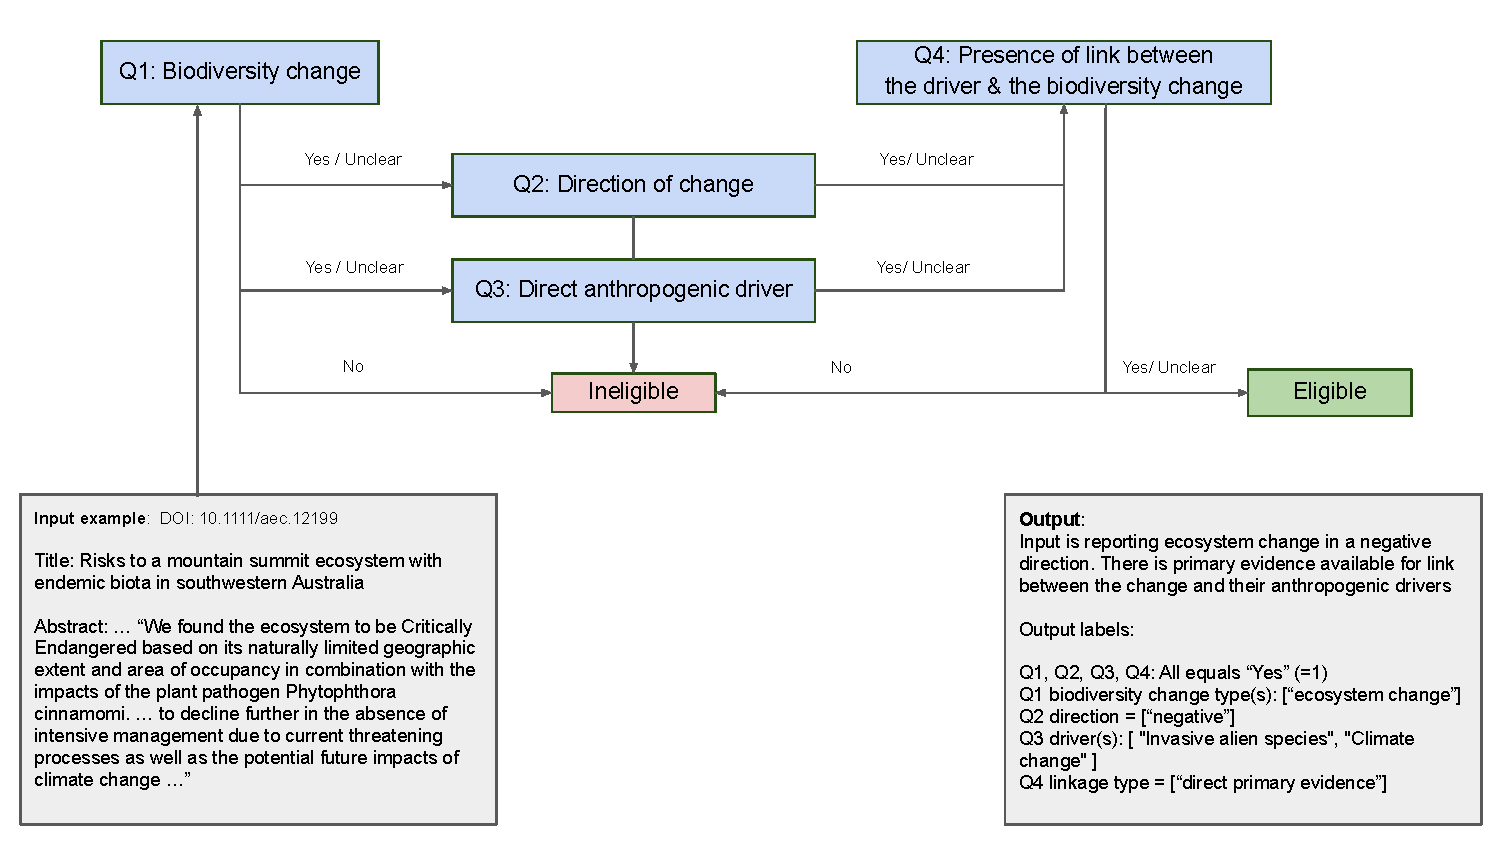
\includegraphics[width=\textwidth]{attachments/screening_process.pdf}
  \caption{\textbf{Eligibility screening procedure:} Each record is screened using four questions (\texttt{Q1}--\texttt{Q4}) applied to its title and abstract. A record is classified as eligible only when all four questions return \texttt{Unclear} or \texttt{Yes}; a single \texttt{No} at any question yields an ineligible classification. Each question produces a structured label alongside its result. See Supplementary Table~\ref{tab:screening_examples} for additional examples.}
  \label{figure:screening_process}
\end{figure}

% % -----------------------------------------------------------
\subsection*{Consistency Checking}
% Describe the process for checking consistency of decisions including the levels at which consistency checking will be undertaken and estimated proportion of articles/studies that will be screened and checked for consistency by two or more reviewers (e.g. Titles (10%), abstracts (10%), full text (100%)). The eligibility criteria should be independently applied by more than one reviewer to a sample of justified size of the screened articles/studies at title, abstract and full text. Replicability of eligibility decisions should be measured and reported and all disagreements between reviewers discussed so that the resolutions informed subsequent assessments. (max. 250 words)
% % -----------------------------------------------------------
Eligibility screening deviates from CEE guidelines in two respects: all decisions will be made by GPT-5-nano rather than multiple human reviewers, and no full-text screening stage will be applied. Both are acknowledged as limitations; their effect on screening reliability will be assessed through two consistency checks against expert full-text labels, defined as eligibility decisions assigned by the original authors of the reference sources based on full-text reading (see Table~\ref{tab:dataset_overview_screening}). As each reference source applies its own inclusion criteria, expert labels may not map perfectly with the eligibility criteria of this map; the alignment between these criteria is treated as a working assumption of the consistency checking procedure.

Consistency Check 1 (CC1) will compare author-assigned labels from abstracts only against expert full-text and LLM labels, establishing a human recall baseline; Consistency Check 2 (CC2) will evaluate LLM labels against expert full-text labels. As screening will be performed by GPT-5-nano, no inter-rater disagreement will arise; reliability will be assessed using recall as the primary metric to minimize false exclusions at the screening step.

% tab:dataset_overview_screening
\begin{table}[H]
\renewcommand{\arraystretch}{1.3}
\setlength{\tabcolsep}{4pt}
\centering
\scriptsize
\begin{tabularx}{\linewidth}{|>{\raggedright\arraybackslash}p{0.22\linewidth}
                             |>{\raggedright\arraybackslash}p{0.12\linewidth}
                             |>{\raggedright\arraybackslash}p{0.30\linewidth}
                             |>{\raggedright\arraybackslash}X|}
\hline
\textbf{Dataset} & \textbf{Size} & \textbf{Details} & 
\textbf{Role} \\
\hline
Reference Screening Dataset & $n = 2{,}418$ & 
Records included in three meta-analyses~\cite{shawetal, kecketal, murphyetal}, a rapid evidence assessment~\cite{jaureguiberry_direct_2022}, and the Red List of Ecosystems Database~\cite{IUCNCEM2022RLE}. & 
CC2: LLM labels evaluated against expert full-text labels to assess screening recall  \\
\hline
Annotated Screening Dataset & $n = 500$ & 
Author-assigned screening labels based on abstracts only, samples drawn from the Reference Screening Dataset and search query results. No full-text access allowed during annotation. & 

CC1: author-assigned labels from abstracts compared against expert full-text and LLM labels, establishing a human recall baseline \\
\hline
\end{tabularx}
\caption{Validation datasets supporting the screening consistency checks.}
\label{tab:dataset_overview_screening}
\end{table}
% -----------------------------------------------------------
\subsection*{Reporting Screening Outcomes}
%% State here how you will report the outcomes of screening (e.g. ROSES diagram plus list of eligible articles plus list of full text articles excluded with reasons for exclusion). (Max 250 words)

% Hunain 20.04.26 - Count = 95

Screening outcomes will be reported in full to support transparency and reproducibility. The following will be provided:

\begin{enumerate}[leftmargin=*]
\item A Reporting Standards for Systematic Evidence Syntheses (ROSES) flow diagram documenting record counts at each stage of the screening pipeline, from raw retrieval to final eligible records.

\item The raw literature retrieval dataset exported from WoS in Parquet format.

\item The full screening output dataset in Parquet format. The field structure is defined in Supplementary Table~\ref{tab:screening_output_fields}.

\item The LLM prompt, model configuration, and raw model output at each eligibility stage for each record.
\end{enumerate}

% -----------------------------------------------------------
\section*{Study Validity Assessment}
%% Describe here the method you propose for critical appraisal of study validity, even this is just by coding of study design (you may include a provisional checklist). An effort may be made to identify other sources of bias relevant to individual included studies (threats to internal and external validity). Each type of bias or threat to internal and external validity should assessed individually for all included studies. You may include a critical appraisal sheet.
% 
% -----------------------------------------------------------
% page 21 - CEE guidelines mentioned that critical appraisal is optional for systematic maps: reads as "Optional (possible if study validityindicators can be captured using thecoding method, but unlikely in practice) –does not influence mapping process itself."
Under CEE guidelines, critical appraisal of study validity is optional for systematic maps and does not influence the mapping process itself. No formal risk-of-bias appraisal will be conducted for exclusion or weighting of included studies. Instead, study validity indicators will be captured through the coding process: study design, data collection method, and analysis method will be coded for every eligible record via the study attributes label set (\texttt{L5}).


% -----------------------------------------------------------
\subsection*{Consistency Checking}
% Describe how repeatability of critical appraisal of study validity will be tested. (Max 250 words)
As no formal critical appraisal is conducted, no dedicated consistency checking for this stage is required. Study validity indicators coded via the study attributes label set (\texttt{L5}) are subject to the coding consistency checks described in the Data Coding Strategy section.

\section*{Data Coding Strategy}
% Describe the method for coding of study metadata (including use of forms/data sheets). (max. 250 words)

% Hunain 20.04.26 - Count = 243
% -----------------------------------------------------------

Eligible records will be coded across six label sets to construct an evidence chain: which drivers are reported as linked to biodiversity change (\texttt{L1}), through which specific threat categories (\texttt{L2}), in which locations and ecosystems (\texttt{L3}; \texttt{L4}), characterized by which study attributes (\texttt{L5}), and affecting which taxa (\texttt{L6}).

All coding decisions will be made by GPT-5-nano (version \texttt{2025-08-07}). The model will code each record by applying pre-defined decision rules to its title and abstract. Prompts will use zero-shot instructions, refined iteratively on training and development splits prior to full-corpus application (see \hyperref[sec:prompts_configs]{Supplementary Text S2} for prompts tuning and freezing procedure).

Where applicable, label sets will draw on controlled vocabularies from established classification schemes: the IPBES Direct Drivers, the IUCN Threats Classification Scheme, IPBES Geographic Regions, the Global Ecosystem Typology (GET), and the GBIF Backbone Taxonomy~\cite{diaz_ipbes_2015,iucn_threats_classification_2022,data_ipbes_geo,keith2022function_get,GBIFBackboneTaxonomy_general}.

Two coding modes will be applied depending on label set structure. Flat-structured label sets (\texttt{L1}, \texttt{L3}, \texttt{L5}) will be coded in a single prompt call per record. Hierarchical label sets (\texttt{L2}, \texttt{L4}) will be coded in staged multiple-pass sequences, where each level's output constrains candidate labels at the next level, avoiding inconsistent assignments. The taxonomy label set (\texttt{L6}) will be applied conditionally: only records flagged by \texttt{L5} as taxon-focused will enter the taxonomy coding step. 

% -----------------------------------------------------------
\subsection*{Metadata to be Coded}
% Describe the variables to be extracted and those that will be coded. (max. 250 words)
% -----------------------------------------------------------
Six label sets will be coded for each eligible record (see output schema in Supplementary Table~\ref{tab:coding_output_fields}).

\emph{IPBES Direct Drivers (\texttt{L1}):} 
broad direct anthropogenic driver category as per the IPBES framework~\cite{diaz_ipbes_2015}.

\emph{IUCN Threats (\texttt{L2}):} 
specific proximate threats to biodiversity, resolved across three hierarchical levels~\cite{iucn_threats_classification_2022}.

\emph{Geographic Scope (\texttt{L3}):} IPBES region, sub-region, and country~\cite{data_ipbes_geo}, together with named sub-national locales and coordinates where reported or inferred from locale names.

\emph{Ecosystem Typology (\texttt{L4}):} Global Ecosystem Typology (GET) realm, biome, and Ecosystem Functional Group~\cite{keith2022function_get}.

\emph{Study Attributes (\texttt{L5}):} 
study design, methods of data collection and analysis, comparator presence and type where reported, and a taxon-focus flag.

\emph{Taxonomy (\texttt{L6}):} 
taxonomic rank, and scope from kingdom to species, resolved against the GBIF Backbone Taxonomy~\cite{GBIFBackboneTaxonomy_general}, applied conditionally to records where \texttt{L5} returns a taxon-focus flag.
% -----------------------------------------------------------
\subsection*{Consistency Checking}
% Describe how repeatability of the meta-data/data extraction process will be tested. At least two people should critically appraise (or cross check appraisal of) each study (max. 250 words)
% -----------------------------------------------------------
Data coding deviates from CEE guidelines in the same two respects as eligibility screening; their effect on coding reliability will be assessed through two consistency checks against expert full-text labels, defined as coded labels assigned by the original authors of the reference sources based on full-text reading (see Table~\ref{tab:dataset_overview_coding}).

Consistency Check 1 (CC1) will compare author-assigned labels from abstracts only against expert full-text labels, establishing a human-performance baseline for each label set; Consistency Check 2 (CC2) will evaluate LLM labels against expert full-text labels across all six label sets (\texttt{L1}--\texttt{L6}). As coding will be performed by GPT-5-nano, no inter-rater disagreement will arise. Reliability will instead be assessed using precision, recall, $F_1$, and Cohen's~$\kappa$.

% tab:dataset_overview_coding
\begin{table}[H]
\renewcommand{\arraystretch}{1.3}
\setlength{\tabcolsep}{4pt}
\centering
\scriptsize
\begin{tabularx}{\linewidth}{|>{\raggedright\arraybackslash}p{0.22\linewidth}
                             |>{\raggedright\arraybackslash}p{0.12\linewidth}
                             |>{\raggedright\arraybackslash}p{0.30\linewidth}
                             |>{\raggedright\arraybackslash}X|}
\hline
\textbf{Dataset} & \textbf{Size} & \textbf{Details} & 
\textbf{Role} \\
\hline
Reference Coding Dataset & $n = 7{,}844$ & 
Records included in three meta-analyses~\cite{benitez-lopez_impact_2017, urban_accelerating_2015, kecketal}, two systematic reviews~\cite{Wrightetal, Lowryetal}, two systematic maps~\cite{moullec_identifying_2025_map, ridleyetal}, a rapid evidence assessment~\cite{jaureguiberry_direct_2022}, and one systematic review preprint~\cite{Pulidoetal}, carrying expert full-text labels across applicable label sets \texttt{L1}--\texttt{L6}. & 
CC2: LLM labels evaluated against expert full-text labels across all six label sets (\texttt{L1}--\texttt{L6}) \\
\hline
Annotated Coding Dataset & $n = 600$ (100 per label set) & 
Author-assigned coding labels based on abstracts only, samples drawn from the 
Reference Coding Dataset. No full-text access allowed during annotation. & 
CC1: labels assigned from abstracts compared against expert full-text labels across all six label sets (\texttt{L1}--\texttt{L6}) \\
\hline
\end{tabularx}
\caption{Validation datasets supporting the data coding consistency checks.}
\label{tab:dataset_overview_coding}
\end{table}
% -----------------------------------------------------------
\section*{Type of Mapping}
% State the type(s) of mapping planned, including provision of metadata and visualisation of the evidence map. (max. 250 words)

% Hunain - 189 words
% -----------------------------------------------------------
This systematic map will be produced as a coded tabular dataset in which 
each row represents one eligible record enriched with labels from all six coding dimensions (\texttt{L1}--\texttt{L6}). Because the pipeline is fully automated and reproducible, the map is designed as a \emph{living systematic map}: it can be re-run against new literature without manual screening and coding.

The dataset will combine a full bibliographic record export from WoS with the metadata fields defined in Supplementary Table~\ref{tab:coding_output_fields}. Full screening outputs will be provided as a separate dataset; the field structure is defined in Supplementary Table~\ref{tab:screening_output_fields}. Both will be made available in a publicly accessible repository alongside the map. The coded dataset will be accompanied by an interactive web application for evidence exploration.

% -----------------------------------------------------------
\subsection*{Narrative Synthesis Methods}
% Describe methods to be used for a narrative synthesis of the evidence base (e.g. in the form of descriptive statistics, tables (including any mapping) and figures). (max. 250 words)
% -----------------------------------------------------------
Narrative synthesis will characterize the distribution of evidence across all six coded dimensions through descriptive statistics on counts and proportions per category. Cross-tabulations of driver by geography, driver by ecosystem, and driver by study attributes will be reported as matrices. Temporal trends in publication volume by driver category will document how the evidence base has evolved since 2000. No effect sizes are estimated and no causal conclusions are drawn.
% Primarily, a systematic map doesn't require effect size, causal conclusion, since these are exploratory exercises, not about making a claim (My note)

% -----------------------------------------------------------
\section*{Knowledge Gap Identification Strategy}
% Describe the methods to be used to identify and/or prioritise key knowledge gaps (unrepresented or underrepresented subtopics that warrant further primary research). (max. 250 words)
% -----------------------------------------------------------
Knowledge gaps will be identified by inspecting cross-tabulation matrices for sparse or absent driver-dimension combinations across geography, ecosystems, study attributes, and taxa. 
% Gap prioritization will draw on IPBES Global Assessment estimates of direct driver importance by geography, ecosystem, and taxa. Combinations where evidence is sparse relative to estimated driver impact represent priority gaps where policy-relevant knowledge is most needed.
% -----------------------------------------------------------
\section*{Demonstrating Procedural Independence}
% Describe the method to ensure review team members, who have also authored articles to be considered within the review, have no role in decisions regarding inclusion or critical appraisal of their own work. (max. 100 words)
% -----------------------------------------------------------
Eligibility screening and data coding will be performed by an LLM pipeline that applies fixed prompts and decision criteria uniformly to all records. Any records authored by review team members will be processed by the same frozen LLM pipeline as all other records; no reviewer discretion will be applied. All pipeline code, prompts, and decision rules will be documented in the supplementary code repository.

% -----------------------------------------------------------
\newpage


\section*{Competing Interests}
% Describe of any financial or non-financial competing interests that the review authors may have. (max. 250 words)
% -----------------------------------------------------------
The authors declare no competing interests.

% -----------------------------------------------------------
\section*{Funding Information}
% All sources of funding for the review should be declared. The proposed role of the funding body in the design of the study and collection, analysis, and interpretation of data and in writing the manuscript should be declared. (max. 250 words)
% -----------------------------------------------------------
No external funding was received.

% -----------------------------------------------------------
\section*{Authors' Contributions}
% The individual contributions of authors to the manuscript should be specified in this section. Please use initials to refer to each author's contribution in this section, for example: "FC analyzed and interpreted the data. RH and AC performed the searching and screening. All authors read and approved the final manuscript." (max. 250 words)
% -----------------------------------------------------------
H.M. developed the protocol and wrote the manuscript. K.F. reviewed the manuscript and provided feedback. S.F. conceived the study, provided supervisory guidance, and reviewed the manuscript. All authors read and approved the final protocol manuscript.


% -----------------------------------------------------------
\section*{Acknowledgements}
% Please acknowledge anyone who contributed towards the article who does not meet the criteria for authorship including anyone who provided professional writing services or materials. Authors should obtain permission to acknowledge from all those mentioned in the Acknowledgements section. (max. 250 words)
% -----------------------------------------------------------
We thank the authors of the published evidence syntheses used to construct the search test list and the validation datasets for screening and coding.
% -----------------------------------------------------------

\section*{Data Availability}
The data repository contains the screening and coding validation 
datasets used to support the consistency checking procedures, 
LLM prompts for all label sets, and 
predefined label classifications with source definitions for each 
label set. All materials are available at: \url{https://osf.io/sna2g/}.


\newpage

% Please use a consistent style for presenting references (max. 500 words)
\bibliography{literature_proceed}


\newpage
\appendix

\section*{Supplementary Tables and Figures}

\setcounter{table}{0}
\setcounter{figure}{0}

\renewcommand{\thetable}{\arabic{table}}
\renewcommand{\thefigure}{\arabic{figure}}
\renewcommand{\tablename}{Supplementary Table}
\renewcommand{\figurename}{Supplementary Figure}
\newpage


% tab:screening_output_fields
\clearpage
\newgeometry{top=0.7cm, bottom=1.0cm, left=1.0cm, right=1.0cm}
\begin{landscape}
\thispagestyle{plain}

\begin{table}[p]
\renewcommand{\arraystretch}{1.04}
\setlength{\tabcolsep}{4pt}
\centering
\scriptsize
\begin{tabularx}{\linewidth}{|>{\raggedright\arraybackslash}p{0.20\linewidth}
                            |>{\raggedright\arraybackslash}p{0.13\linewidth}
                            |>{\raggedright\arraybackslash}X|}
\hline
\textbf{Field} & \textbf{Type} & \textbf{Description} \\
\hline

\multicolumn{3}{|l|}{\textit{Record identifiers and processing metadata}} \\
\hline
\texttt{custom\_id} & String & Unique identifier for the record in the original literature retrieval. \\
\hline
\texttt{\_source\_run} & String & Identifier for the processing partition in which the record was screened. \\
\hline
\texttt{model} & String & Name of the LLM used to generate the screening output. \\
\hline
\texttt{created\_at} & Datetime & Timestamp indicating when the record was processed. \\
\hline
\texttt{raw\_output} & String & Original LLM response before parsing into structured fields. \\
\hline

\multicolumn{3}{|l|}{\textit{Screening outputs \texttt{Q1}--\texttt{Q4}}} \\
\hline
\texttt{q1\_r} & Integer & Q1 result: biodiversity change reported? $1$ = Yes, $-1$ = Unclear, $0$ = No. \\
\hline
\texttt{q1\_label} & List[String] & Biodiversity change type(s): genetic change, species change, community change, or ecosystem change. \\
\hline
\texttt{q2\_r} & Integer & Q2 result: direction identifiable? $1$ = Yes, $-1$ = Unclear, $0$ = No. \\
\hline
\texttt{q2\_label} & List[String] & Direction label(s): negative, positive, mixed, or unclear. \\
\hline
\texttt{q3\_r} & Integer & Q3 result: direct anthropogenic driver mentioned or plausibly implied? $1$ = Yes, $-1$ = Unclear, $0$ = No. \\
\hline
\texttt{q3\_label} & List[String] & Driver or threat name(s) identified during screening; these support eligibility screening and are not the final coding outputs. \\
\hline
\texttt{q4\_r} & Integer & Q4 result: driver--biodiversity link reported or plausibly implied? $1$ = Yes, $-1$ = Unclear, $0$ = No. \\
\hline
\texttt{q4\_label} & List[String] & Linkage type(s) describing how the driver is linked to the reported biodiversity change. \\
\hline

\multicolumn{3}{|l|}{\textit{Eligibility decision}} \\
\hline
\texttt{pred\_screening} & List[String] & Final eligibility decision derived from \texttt{Q1}--\texttt{Q4}: \texttt{["ELIGIBLE"]} or \texttt{["INELIGIBLE"]}. \\
\hline

\multicolumn{3}{|l|}{\textit{Bibliographic details}} \\
\hline
\texttt{Article Title} & String & Title of the bibliographic record. \\
\hline
\texttt{Abstract} & String & Abstract of the bibliographic record. \\
\hline
\texttt{Publication Year} & Integer & Publication year of the bibliographic record. \\
\hline
\texttt{Authors} & String & Authors of the bibliographic record. \\
\hline
\texttt{DOI} & String & DOI of the bibliographic record, where available. \\
\hline

\end{tabularx}
\vspace{2pt}
\caption{\textbf{Output fields recorded for each record in the screening dataset:} Screening fields (\texttt{Q1}--\texttt{Q4}) record the decision result and structured label(s) generated for each eligibility question.}
\label{tab:screening_output_fields}
\end{table}

\end{landscape}
\restoregeometry
\clearpage

% tab:screening_examples
\newgeometry{top=0.5cm, bottom=1.5cm, left=1cm, right=1cm}
\thispagestyle{plain}
\begin{landscape}
\begin{table}[p]
\renewcommand{\arraystretch}{1.0}
\setlength{\tabcolsep}{3pt}
\centering
\singlespacing 
\scriptsize
\begin{tabularx}{\linewidth}{|>{\raggedright\arraybackslash}p{0.02\linewidth}
                             |>{\raggedright\arraybackslash}p{0.11\linewidth}
                             |>{\raggedright\arraybackslash}p{0.16\linewidth}
                             |>{\raggedright\arraybackslash}p{0.08\linewidth}
                             |>{\raggedright\arraybackslash}p{0.05\linewidth}
                             |>{\raggedright\arraybackslash}p{0.10\linewidth}
                             |>{\raggedright\arraybackslash}p{0.07\linewidth}
                             |>{\raggedright\arraybackslash}p{0.06\linewidth}
                             |>{\raggedright\arraybackslash}X|}
\hline
\textbf{\#} &
\textbf{Title} &
\textbf{Abstract excerpt} &
\textbf{Q1: Change} &
\textbf{Q2: Dir.} &
\textbf{Q3: Driver(s)} &
\textbf{Q4: Linkage} &
\textbf{Decision} &
\textbf{Rationale} \\
\hline

1 &
Risks to a mountain summit ecosystem with endemic biota in southwestern Australia &
``\ldots We found the ecosystem to be Critically Endangered based on its naturally limited geographic extent and area of occupancy in combination with the impacts of the plant pathogen \textit{Phytophthora cinnamomi}. \ldots'' &
Ecosystem change &
Negative &
Invasive alien species; Climate change &
Direct primary evidence &
\textbf{Eligible} &
Reports ecosystem-level change in a negative direction, identifies two anthropogenic drivers, and provides direct empirical evidence linking them to the change. \\
\hline

2 &
Vulnerability of Antarctic shallow invertebrate-dominated ecosystems &
``\ldots Climate change is likely to cause early breakout of seasonal sea ice \ldots This is predicted to result in ecological regime shifts, in which invertebrate-dominated communities are replaced by macroalgal beds \ldots'' &
Ecosystem change; Community change &
Negative &
Climate change &
Projected &
\textbf{Eligible} &
Reports both ecosystem- and community-level change, with regime shifts framed as negative. Linkage is projected because the driver--biodiversity connection is based on predicted future scenarios. \\
\hline

3 &
The effects of grazing and watering on ecosystem CO\textsubscript{2} fluxes vary by community phenology &
``\ldots Grazing profoundly influences vegetation and the subsequent carbon fluxes in various ecosystems \ldots little effort has been made to explore the underlying mechanisms for phenological changes and their consequences on carbon fluxes at ecosystem level.'' &
Ecosystem change &
Both positive and negative directions identified &
Grazing; Watering &
Direct primary evidence &
\textbf{Eligible} &
The study examines anthropogenic grazing and watering effects on desert steppe and ecosystem carbon fluxes. The driver-change relationship is directly assessed through experiments. \\
\hline

4 &
Modeling Carbon Stocks in a Secondary Tropical Dry Forest in the Yucatan Peninsula, Mexico &
``\ldots The carbon balance of secondary dry tropical forests is sensitive to human and natural disturbances and climate change \ldots Carbon stocks were largely influenced by human disturbances between 1985 and 2010.'' &
No change reported &
No direction of change identified &
Human disturbances; Climate change &
No linkage present &
\textbf{Ineligible} &
Although anthropogenic drivers are identified, the study focuses on carbon stocks rather than biodiversity change. \\
\hline

\end{tabularx}
\caption{Examples of the screening procedure.}
\label{tab:screening_examples}
\end{table}
\end{landscape}
\restoregeometry


% tab:coding_output_fields
\newpage
\newgeometry{top=0.8cm, bottom=1.5cm, left=1cm, right=1cm}
\thispagestyle{plain}
\begin{landscape}
\begin{table}[p]
\renewcommand{\arraystretch}{1.15}
\setlength{\tabcolsep}{4pt}
\centering
\scriptsize
\begin{tabularx}{\linewidth}{|>{\raggedright\arraybackslash}p{0.25\linewidth}
                             |>{\raggedright\arraybackslash}p{0.13\linewidth}
                             |>{\raggedright\arraybackslash}X|}
\hline
\textbf{Field} & \textbf{Type} & \textbf{Description} \\
\hline

\multicolumn{3}{|l|}{\textit{L1: IPBES Direct Drivers}} \\
\hline
\texttt{driver} & List[String] & IPBES direct driver category or categories assigned to the record. \\
\hline

\multicolumn{3}{|l|}{\textit{L2: IUCN Threats}} \\
\hline
\texttt{pred\_threat\_l0} & List[String] & Broadest IUCN Threats Classification level assigned to the record. \\
\hline
\texttt{pred\_threat\_l1} & List[String] & Intermediate IUCN Threats Classification level assigned to the record. \\
\hline
\texttt{pred\_threat\_l2} & List[String] & Most specific IUCN Threats Classification level assigned to the record. \\
\hline

\multicolumn{3}{|l|}{\textit{L3: Geography}} \\
\hline
\texttt{pred\_regions} & List[String] & IPBES region or regions of study focus. \\
\hline
\texttt{pred\_subregions} & List[String] & IPBES sub-region or sub-regions of study focus. \\
\hline
\texttt{pred\_countries} & List[String] & Countries of study focus, recorded using ISO 3166-1 alpha-3 codes. \\
\hline
\texttt{locales} & List[String] & Free-text names of sub-national locations mentioned in the title or abstract, such as parks, reserves, cities, or mountain ranges. \\
\hline
\texttt{locale\_coordinates} & List[List[Float]] & [latitude, longitude] pairs in decimal degrees (WGS84, EPSG:4326); resolved from explicit coordinates in the title or abstract, or inferred from the locale name if absent. \\
\hline

\multicolumn{3}{|l|}{\textit{L4: Ecosystem Typology}} \\
\hline
\texttt{pred\_realm} & List[String] & Global Ecosystem Typology realm or realms of study focus. \\
\hline
\texttt{pred\_biome} & List[String] & Global Ecosystem Typology biome or biomes of study focus. \\
\hline
\texttt{pred\_efg} & List[String] & Global Ecosystem Typology Ecosystem Functional Group or groups of study focus. \\
\hline

\multicolumn{3}{|l|}{\textit{L5: Study Attributes}} \\
\hline
\texttt{pred\_study\_design} & String & Study design category: Observational, Experimental, Modeling, or Unclear. \\
\hline
\texttt{pred\_methods\_data\_collection} & List[String] & Data collection method or methods reported in the title or abstract, where applicable. \\
\hline
\texttt{pred\_methods\_analysis} & List[String] & Analysis method or methods reported in the title or abstract, where applicable. \\
\hline
\texttt{pred\_has\_comparison} & Boolean & True if the record explicitly states or strongly implies a comparator, such as pre/post, control versus exposed sites, or reference sites; otherwise false. \\
\hline
\texttt{pred\_comparison\_types} & List[String] & Type or types of comparison identified for the record, where applicable. \\
\hline
\texttt{pred\_taxa} & Boolean & True if the record focuses on one or more specific taxonomic groups; otherwise false. \\
\hline

\multicolumn{3}{|l|}{\textit{L6: Taxonomy} (\textit{conditional on} \texttt{pred\_taxa = True})} \\
\hline
\texttt{rank} & List[String] & Lowest taxonomic rank(s) identified for the focal taxon name(s) in the title or abstract. \\
\hline
\texttt{kingdom} & List[String] & Kingdom(s) resolved through the GBIF Backbone Taxonomy. \\
\hline
\texttt{phylum} & List[String] & Phylum/phyla resolved through the GBIF Backbone Taxonomy. \\
\hline
\texttt{class} & List[String] & Class(es) resolved through the GBIF Backbone Taxonomy. \\
\hline
\texttt{order} & List[String] & Order(s) resolved through the GBIF Backbone Taxonomy. \\
\hline
\texttt{family} & List[String] & Family/families resolved through the GBIF Backbone Taxonomy. \\
\hline
\texttt{genus} & List[String] & Genus/genera resolved through the GBIF Backbone Taxonomy. \\
\hline
\texttt{species} & List[String] & Species resolved through the GBIF Backbone Taxonomy. \\
\hline
\end{tabularx}
\vspace{4pt}
\caption{\textbf{Coded output fields for each eligible record across six label sets (\texttt{L1}--\texttt{L6}):} \texttt{L6} is applied conditionally to records where \texttt{pred\_taxa = True} in \texttt{L5}. Where a field is not warranted by the record's scope, \texttt{"Not Applicable"} is coded; where a label cannot be determined from the title or abstract, \texttt{"Unclear"} is coded.}
\label{tab:coding_output_fields}
\end{table}
\end{landscape}
\restoregeometry

\newpage

% figure:conceptual_model
% Theory of change / conceptual model
% Provide a theory of change and/or conceptual model that describes the hypothesised link(s) between the intervention/exposure to the outcome(s). Use either text or attach graphic as an additional file.
\begin{figure}[htbp]
  \centering
  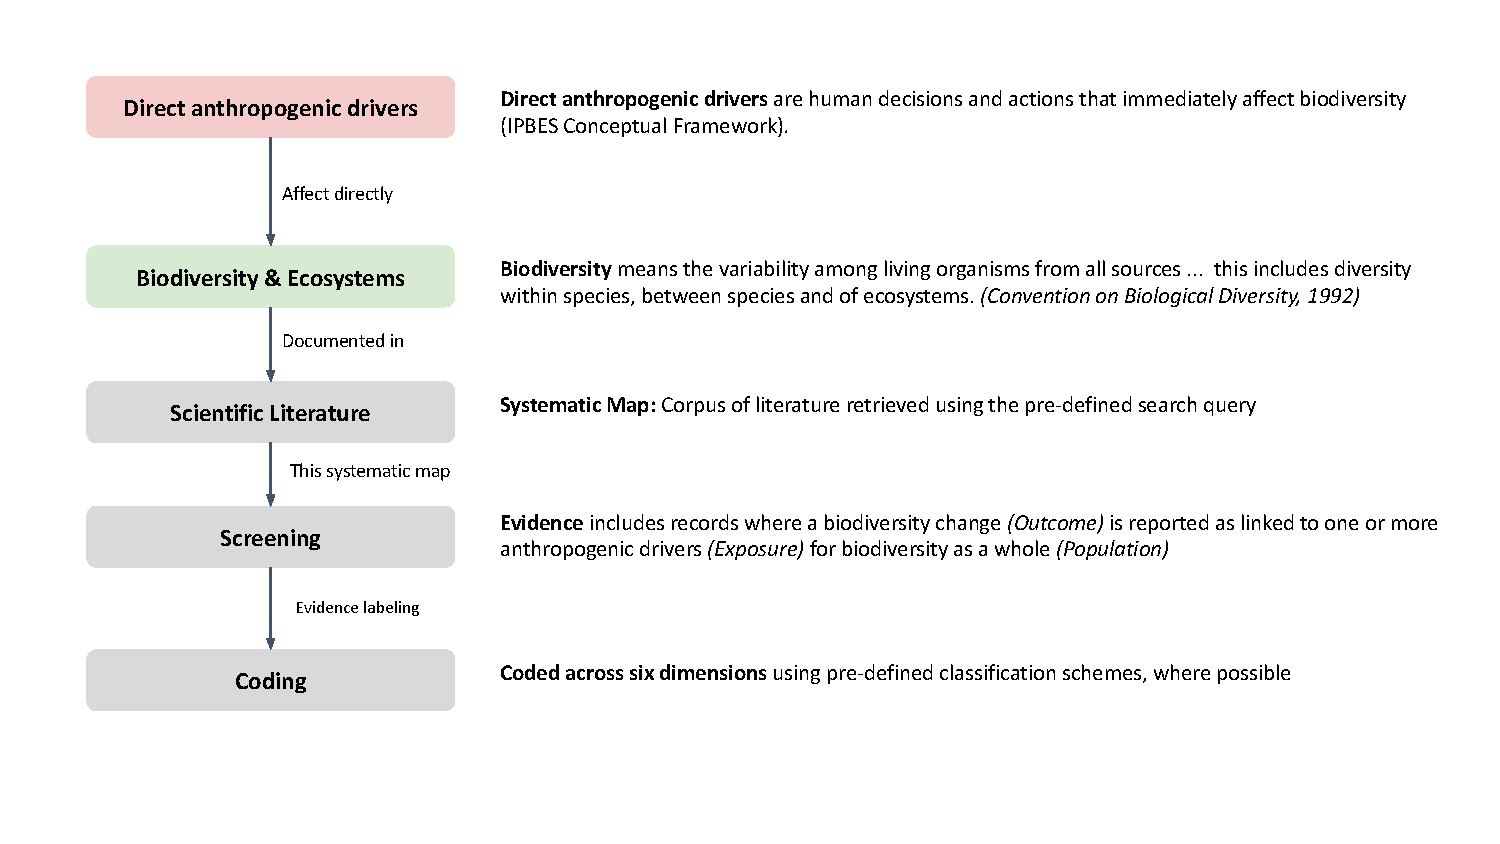
\includegraphics[width=0.90\textwidth]{attachments/theory_of_change_proceed.pdf}
  \singlespacing 

\caption{\textbf{Conceptual Model}: Direct anthropogenic drivers are human decisions and actions that immediately affect biodiversity (IPBES Conceptual Framework). Scientific literature reporting biodiversity change linked to these drivers is retrieved via a systematic search, screened for eligibility, and coded across six dimensions using pre-defined classification schemes.}
  \label{figure:conceptual_model}
\end{figure}








\newpage


\section*{Supplementary Text S1}
\phantomsection\label{sec:biodiversity_loss_evidence} 

Biodiversity, as defined under the Convention on Biological Diversity (CBD) and operationalized by IPBES, encompasses the variability among living organisms from all sources, including terrestrial, marine, and other aquatic ecosystems, and the ecological complexes of which they are part. This includes diversity within species, between species, and of ecosystems~\cite{CBD1992,spm_ga_ipbes_2019}. In this systematic map, eligibility is based on evidence of biodiversity change, while the primary analytical focus is biodiversity loss. Evidence is operationalized through four components: a reported biodiversity change, the direction of that change, an anthropogenic driver linked to it, and the nature of the link between them.

\paragraph*{Biodiversity change:}
Biodiversity change may be reported in one or more of four broad forms:
\begin{enumerate}
    \item \emph{Genetic change}: such as change in genetic diversity or 
    other heritable variation within a species or population;
    \item \emph{Species change}: such as change in the abundance, 
    occupancy, distribution, persistence, or extinction risk of a taxon, 
    species, or population;
    \item \emph{Community change}: such as change in richness, evenness, 
    turnover, homogenization, or composition of a species assemblage; and
    \item \emph{Ecosystem change}: such as change in ecosystem structure, 
    function, integrity, extent, connectivity, or collapse risk.
\end{enumerate}

These four forms operationalize the CBD definition at different levels of biological organization in this systematic map. Genetic change corresponds to biodiversity \emph{within species}; species change and community change together capture important ways in which biodiversity \emph{between species} is reported in the literature; and ecosystem change captures biodiversity \emph{of ecosystems}~\cite{CBD1992}. The forms are not mutually exclusive: a single study may report change at more than one level.

\paragraph*{Direction of change:}
Biodiversity change may be negative (decline, degradation, loss), positive (recovery, restoration, increase), mixed, or unclear. The analytical focus of this systematic map is on biodiversity loss, that is, negative change in the state of biodiversity at one or more of these levels. Records reporting other directions of change are retained and coded but treated separately during synthesis.

\paragraph*{Direct anthropogenic drivers:}
Biodiversity change must be linked to at least one direct anthropogenic driver. The broad driver categories follow the IPBES conceptual framework: land/sea-use change, direct exploitation and resource extraction, climate change, pollution, and invasive alien species~\cite{diaz_ipbes_2015}. Specific human activities and pressures within these categories are further characterized using the IUCN Threats Classification Scheme~\cite{iucn_threats_classification_2022}, which provides a hierarchical vocabulary of proximate threats to biodiversity.

\paragraph*{Linkage:}
A record constitutes evidence when it reports or implies a link between one or more direct anthropogenic drivers and the reported biodiversity change. This link may take different forms, ranging from direct empirical observation to model-based projection, and its nature is recorded as part of the screening output.

Together, these four components define what this systematic map treats as evidence: a study that reports biodiversity change, describes its direction, identifies an anthropogenic driver, and connects the two. The Screening Strategy section describes how these components are operationalized into inclusion and exclusion decisions.
\newpage


\section*{Supplementary Text S2}
\phantomsection\label{sec:prompts_configs}

\textbf{Prompts:} Prompts for screening and all label sets are provided in the data repository (see Data Availability section). Each prompt specifies a constrained set of output labels; for the majority of label sets, these are derived from established classification schemes: IPBES Direct Drivers (\texttt{L1}), IUCN Threats Classification (\texttt{L2}), IPBES Geography (\texttt{L3}), Global Ecosystem Typology (\texttt{L4}), and GBIF Taxonomy (\texttt{L6}). Label definitions and decision rules are adopted from source materials; for instance, IUCN threat definitions and notes are incorporated verbatim. The data repository provides the full label inventory with source definitions for each label set. Prompts will be further refined iteratively on the training split. Final configurations will be frozen prior to full-corpus application.

\textbf{Parameters:} Only reasoning effort will be varied during tuning. The reasoning effort setting will be selected on the development split.

\textbf{Data Splits:} The validation datasets are partitioned into training (60\%), development (20\%), and test (20\%) splits using stratified sampling with a fixed random seed, stratified by label column and original label sources. The training split was used for initial prompt development and will be used for further prompt refinement; the development split will be used for model selection and reasoning effort tuning; the test split will be held out for final consistency checking prior to full-corpus application.

\textbf{Freezing Condition:} Prompts and reasoning effort will be refined iteratively. After each iteration, consistency checking metrics described in the Consistency Checking sections will be evaluated on training and development splits. Configurations will be frozen when no significant improvement in these metrics is observed across iterations. Prior to full-corpus application, a final evaluation on the held-out test split will be conducted to confirm consistency checking results.

\end{document}
